% ======================================================================
\section{Experiments}
\label{sec:exp}

\paragraph{Metrics.}
A drift estimate in the embedding is compared with the \emph{push-forward}
of the true input velocity into that same embedding, $J_iv_i$, with the
Jacobian $J_i$ of the map estimated by local linear regression of embedded
offsets on tangent-projected input offsets. \emph{Direction} is the mean
cosine between the two (points above the 20th percentile of reference
speed); \emph{speed} is the Spearman correlation of their norms;
\emph{kNN} is the fraction of each point's 10 input neighbours kept in the
layout. When a ground-truth order exists (developmental stage, cell-cycle
phase), we also run the Markov chain of the embedding's own kernel,
$Q_{ij}/\sum_kQ_{ik}$ restricted to $k$ neighbours, and report how far $s$
steps progress along that order, relative to the chain of a symmetric
embedding of the same data with the same neighbours (\emph{progress}).
This measures whether the directed structure seen in the map is supported
by the data, which projected arrows cannot do.

% ----------------------------------------------------------------------
\subsection{Synthetic flows}
\label{sec:exp_toy}

\paragraph{Data.}
\emph{Sphere vortex}: $n=1500$ points uniform on $S^2\subset\R^3$, with
the rotation $v(x)=e_z\times x$, divergence-free with two centres at the
poles. \emph{Swiss roll}: $n=1500$, $v$ the unit tangent along the roll, a
gradient drift. \emph{Noisy cycle}: $n=1500$, a mixed drift in high
dimension. In a 2-D latent space, two thirds of the points lie on an
attracting ring (rotation plus a pull $-2(r-1)$ towards $r=1$) and the rest
on a branch leaving it tangentially, travelled at unit speed. A fixed smooth
map $u\mapsto Q\,[u,\tfrac12\sin(Wu+b)]$ (6 random features, $Q$ an
orthonormal $50\times8$ frame) lifts both to $\R^{50}$, with $v$ pushed
forward by its Jacobian. Isotropic noise is then added to the points
(norm $1.5\times$ the median 10-NN distance) and, independently, to the
velocities (norm $1\times$ their median). After noise, the input's 10-NN
keep $0.64$ of the latent ones and the velocity has cosine $0.69$ with its
clean value; references are computed from the clean latent. Every method
receives the same averaged Randers cost ($\rho=0.9$); 3 seeds.

\paragraph{Baselines.}
Symmetric t-SNE fitted to the same balanced input affinity (direction-blind
control). Finsler MDS \citep{dages2025finsler}, with the authors' corrected
SMACOF, on the directed graph geodesics of the same Randers edge costs
(10-NN graph), as in their Swiss-roll experiments. Finsler t-SNE
\citep{dages2026harnessing}, which has no public code: we reimplement it as
the Student kernel on the canonical Randers cost, with a constant drift
$\alpha e_2$ and the row-stochastic input, fitted with FlowSNE's optimiser.
For both, $\alpha$ is chosen in $\{0,0.2,\dots,0.8,0.9\}$ by the method's
own objective (stress, cross-entropy). The directed diffusion embedding of
\citet{debaussart2026finslerian}, with their code and graph construction,
embeds with Isomap and estimates the drift by applying the antisymmetric
operator to the layout coordinates. FlowSNE is run jointly and, as an
ablation, with the layout frozen at the symmetric t-SNE layout of the same
affinity, fitting only the field (drift-only, \cref{sec:kernel}).

\begin{table*}[t]
  \caption{Synthetic flows, mean over 3 seeds (spread $\le0.03$, except speed,
  $\le0.07$). Direction and speed compare each method's drift with the
  push-forward of the true drift into its own layout; a constant drift has no
  speed. kNN: 10-NN preservation, Euclidean in both spaces (direction-blind).
  kNN$_\to$: overlap of the 10 nearest \emph{targets} under the input Randers
  cost and under the method's own output cost (Euclidean for the symmetric and
  Isomap layouts). $^\dagger$Finsler MDS selects $\alpha=0$ on
  the sphere: no drift.}
  \label{tab:toy}
  \centering
  \small
  \setlength{\tabcolsep}{3.5pt}
  \begin{tabular}{lccccccccccc}
    \toprule
    & \multicolumn{4}{c}{sphere vortex (circulation)} & \multicolumn{3}{c}{Swiss roll (gradient)}
    & \multicolumn{4}{c}{noisy cycle in $\R^{50}$ (mixed)} \\
    \cmidrule(lr){2-5}\cmidrule(lr){6-8}\cmidrule(lr){9-12}
    method & dir. & speed & kNN & kNN$_\to$ & dir. & kNN & kNN$_\to$ & dir. & speed & kNN & kNN$_\to$ \\
    \midrule
    symmetric t-SNE & -- & -- & 0.68 & 0.58 & -- & 0.66 & 0.46 & -- & -- & \textbf{0.68} & 0.34 \\
    Finsler MDS \citep{dages2025finsler} & --$^\dagger$ & -- & 0.45 & 0.38 & \textbf{1.00} & \textbf{0.94} & \textbf{0.86} & 0.25 & -- & 0.56 & 0.27 \\
    Finsler t-SNE \citep{dages2026harnessing} & 0.80 & -- & 0.78 & 0.79 & 0.91 & 0.83 & 0.79 & 0.79 & -- & 0.66 & 0.52 \\
    Debaussart-Joniec et al., Isomap & \textbf{0.98} & 0.61 & 0.48 & 0.31 & 0.97 & 0.86 & 0.36 & 0.93 & 0.41 & 0.51 & 0.24 \\
    FlowSNE, balanced, frozen layout & 0.85 & 0.40 & 0.68 & 0.71 & 0.81 & 0.66 & 0.63 & 0.92 & $-0.25$ & \textbf{0.68} & 0.50 \\
    FlowSNE, balanced input & 0.95 & \textbf{0.85} & \textbf{0.81} & \textbf{0.82} & 0.98 & 0.75 & 0.70 & 0.95 & 0.63 & 0.67 & 0.53 \\
    FlowSNE, row-stochastic input & 0.95 & 0.76 & 0.79 & 0.80 & 0.99 & 0.80 & 0.82 & \textbf{0.98} & \textbf{0.81} & 0.67 & \textbf{0.61} \\
    \bottomrule
  \end{tabular}
\end{table*}

\begin{figure*}[t]
  \centering
  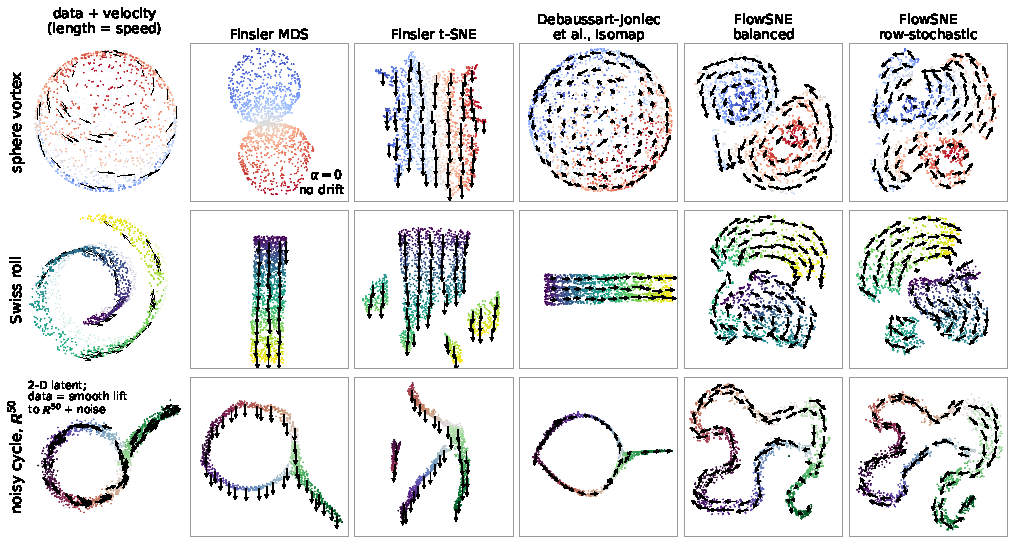
\includegraphics[width=\textwidth]{figures/table2_layouts.pdf}
  \caption{Layouts of the methods of \cref{tab:toy} (seed 0). First column:
  the data in $\mathbb{R}^3$ with the true velocity, arrow length
  proportional to speed (zero at the poles; unit speed on the Swiss roll);
  for the noisy cycle, which lives in $\R^{50}$, its 2-D latent with the
  clean velocity. Sphere coloured by height (red north, blue south), Swiss
  roll by its roll parameter, noisy cycle by phase on the ring (cyclic map)
  and by arclength on the branch (greens). Arrows: each method's drift in flow direction, averaged per
  grid cell, length relative to the panel's largest arrow (units differ
  between methods).}
  \label{fig:toy_layouts}
\end{figure*}

\paragraph{Results.}
\Cref{tab:toy,fig:toy_layouts}. A constant drift is the gradient of a linear potential, so
the two canonical-Randers baselines can only express progress along one
axis. On the Swiss roll, whose drift is a gradient, Finsler MDS on geodesic
distances unrolls the roll and is best in every column, as Isomap already is
for the layout; FlowSNE with a row-stochastic input matches its direction
($0.99$) but tears the roll into pieces. On the sphere the drift is a pure
circulation. Finsler MDS selects $\alpha=0$; Finsler t-SNE can use its drift
only by cutting the sphere along a meridian and unrolling it into a strip,
where the rotation becomes a translation (direction $0.80$), and it fits its
own objective worse than FlowSNE on the same input (cross-entropy $11.89$
against $11.62$). FlowSNE recovers the rotation ($0.95$) with the best speed
and the best neighbourhoods, directed or not; its layout keeps more
neighbours than the symmetric fit of the same affinity ($0.81$ against
$0.68$). The directed diffusion embedding is best in direction on its
Isomap layout, which keeps the fewest neighbours. On the sphere, the fitted
field has two vortex centres, on the images of the two poles
(\cref{app:toy}). The frozen-layout ablation shows what the joint fit
buys: a field fitted on the symmetric layout still finds the direction
($0.81$--$0.92$), but its speeds are wrong (Spearman $0.40$ on the sphere,
$-0.25$ on the cycle, against $0.85$ and $0.63$) and its directed
neighbourhoods stop halfway between the symmetric and the joint layout. The
direction can be painted onto a symmetric map; the speeds and the directed
neighbourhoods need the layout to move.

The noisy cycle mixes both cases in high dimension. A constant drift can
follow only one part of a ring: Finsler MDS selects $\alpha=0.2$ (direction
$0.25$), and Finsler t-SNE again cuts the ring and stacks the pieces along
its drift ($0.79$). FlowSNE recovers the mixed drift with the
row-stochastic input (direction $0.98$, speed $0.81$, kNN$_\to$ $0.61$, best
in all three) and slightly less well with the balanced one ($0.95$, $0.63$,
$0.53$), which hides the gradient parts, the pull towards the ring and the
branch. Its layouts keep as many neighbours as the symmetric fit ($0.67$
against $0.68$; the input's own 10-NN keep $0.64$ of the latent ones) and
stay connected, but draw the ring as a thin meandering line where every
direction-blind method draws a circle. This is the objective, not the
lift or the optimiser (\cref{app:fold}): a drift of norm near $\rho$
discounts forward distances, so the joint fit stretches the layout along
the flow ($1.6\times$ the symmetric ring's length for the same canvas) and
thins it, and a stretched loop in the plane meanders. Lowering $\rho$ to
$0.5$ unfolds it but destroys the speed ranking; starting the joint fit
from the symmetric layout instead of PCA reaches a lower loss and a
rounder ring with the same direction and speed. The directed diffusion
embedding is close in direction ($0.93$) but ranks speeds worse ($0.41$).


% ----------------------------------------------------------------------
\subsection{Single-cell RNA velocity}
\label{sec:exp_sc}

\paragraph{What this section tests.}
\Cref{sec:gauge} predicts that the two input affinities see different
parts of a drift: a balanced affinity sees only its cyclic part, a
row-stochastic one also its gradient part, together with the density of
the data (eq.~\ref{eq:firstorder}: it rewards a field that points at the
points with many neighbours). Three claims follow, which we test on data
where the true order of the points is known from outside the data.
(i) When the drift is mostly a gradient, the row-stochastic input is the
right one and balancing loses the signal. (ii) When the drift circulates,
the balanced input isolates the circulation, while the row-stochastic one
fits the density instead and produces a spurious field. (iii) An
embedding can lose directed information but not create it: the chain of a
map progresses at most as far as the chain of the input.

\paragraph{Data.}
Each sample is a cell, described by its gene-expression vector reduced to
30 principal components. \emph{RNA velocity} is an estimate, for every
cell, of where its expression is heading in the next hours, obtained from
the mRNA that is still being produced \citep{lamanno2018rna} or from mRNA
labelled by its age; it is a noisy vector per cell, in the same 30
coordinates. The Hodge share of \cref{sec:gauge}, computed on the 30-NN
graph, says which regime a dataset is in.
\emph{Pancreas} \citep{bastidasponce2019comprehensive} ($n=3696$,
velocity from scVelo \citep{bergen2020generalizing}): progenitor cells
mature into four hormone-producing types, a one-way process; the velocity
is $83\%$ gradient. \emph{Cell cycle} \citep{battich2020sequencing}
($n=2793$, velocity from dynamo's labelled mRNA): a human cell line in
which cells grow, copy their DNA and divide, over and over, so the
expression state moves around a loop. Two fluorescent markers, read on
each cell independently of its expression, give its position on that
loop as a number in $[0,1)$: a ground-truth phase that no method has
seen. The loop is not quite closed in the data: the cells about to divide
(the last twelfth of the loop, ``late M'') have almost no neighbours among
the cells that have just divided ($1\%$ of their 15-NN), so the loop is an
arc, and progress through its seam is the hardest test. The velocity is
$67\%$ gradient, but that part walks \emph{backwards} in phase ($-0.06$
cycle in 25 steps) and the cyclic part forward ($+0.26$): the circulating
content is exactly what balancing keeps. \emph{Gastrulation}
\citep{pijuansala2019single} ($n=30\,000$, KeOps) is the scale test; its
order is the real age of the embryo each cell was taken from.

\paragraph{Gradient regime: pancreas.}
Here the row-stochastic input is the right one (claim i): the field
FlowSNE fits agrees with the standard practice, the velocity projected
onto the map, at $0.76$ (balanced input: $0.54$), and keeps a better
layout than the directed diffusion embedding on its Isomap layout (kNN
$0.50$ against $0.29$, direction $0.69$). On gastrulation (claim iii), 25 steps of the
chain of the input affinity progress $0.37$ days further in embryo age than
a direction-blind chain, close to scVelo's own transition kernel ($0.39$);
the chain of a 10-D FlowSNE embedding keeps $0.30$ days of it, that of a
2-D map $0.13$: a map loses part of the directed information, it does not
add to it.

\begin{figure}[t]
  \centering
  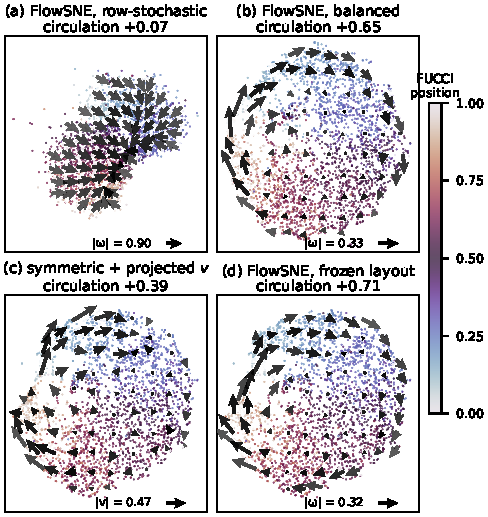
\includegraphics[width=\columnwidth]{figures/rpe1_maps.pdf}
  \caption{Cell cycle, 2-D maps, coloured by the measured phase (cyclic
  colour map, so the two ends of the scale are the same point of the loop);
  arrows: mean field per grid cell, length relative to each panel's own
  reference value (key; the row-stochastic field is saturated at $0.9$,
  the balanced ones sit near $0.1$--$0.3$). (a) Fitted jointly to the row-stochastic affinity, the field
  saturates at its bound and converges on the dense centre of the map: it
  fits the density, a gradient (eq.~\ref{eq:firstorder}), and the layout
  loses its neighbourhoods. (b) To the balanced affinity, it is
  unsaturated and circulates around the loop. (c) The symmetric layout of
  the balanced affinity with the velocity projected onto it, the standard
  practice. (d) FlowSNE with the layout frozen at (c): only the field is
  fitted, to the same balanced affinity as (b); it gives the same
  circulation as (b), on the symmetric layout.}
  \label{fig:rpe1}
\end{figure}

\begin{table}[t]
  \caption{Cell cycle, 2-D and 10-D maps (FlowSNE: 3 seeds; symmetric and
  frozen layout: seed 0). Every row uses the balanced affinity except the
  row-stochastic one. Frozen layout: the symmetric map is kept fixed and
  only the field $\omega$ is fitted, on the same loss as the joint fit.
  Circ.: does the map's field go around the loop? Net over absolute flow of
  the field around 200 loops through the 12 phase bins of the map's own
  30-NN graph ($1$: always forward, $0$: a gradient). Progress: measured
  phase gained in 10 steps of a walk that follows the field, over the same
  walk ignoring it, in cycles; late M: the same for the cells about to
  divide, which must cross the seam. kNN: 10-NN preservation, Euclidean.
  The input velocity itself, in 30 dimensions, scores $0.19$, $0.088$,
  $0.15$.}
  \label{tab:rpe1}
  \centering
  \small
  \setlength{\tabcolsep}{4pt}
  \begin{tabular}{lcccc}
    \toprule
    map / field & circ. & progress & late M & kNN \\
    \midrule
    \multicolumn{5}{l}{\emph{2-D}} \\
    symmetric + projected $v$ & 0.39 & 0.028 & 0.04 & \textbf{0.22} \\
    FlowSNE, row-stochastic & 0.07 & 0.032 & $-0.12$ & 0.09 \\
    FlowSNE, balanced & 0.68 & 0.075 & 0.08 & 0.15 \\
    FlowSNE, bal., frozen layout & \textbf{0.69} & \textbf{0.082} & \textbf{0.13} & \textbf{0.22} \\
    \midrule
    \multicolumn{5}{l}{\emph{10-D}} \\
    symmetric + projected $v$ & \textbf{0.35} & 0.048 & 0.05 & \textbf{0.30} \\
    FlowSNE, row-stochastic & 0.13 & 0.166$^\ast$ & $-0.08$ & 0.27 \\
    FlowSNE, balanced & 0.31 & 0.059 & \textbf{0.15} & 0.28 \\
    \bottomrule
  \end{tabular}
  \par\smallskip\raggedright\footnotesize
  $^\ast$A density artefact: the field points at the dense regions, which
  happen to lie forward in phase for most cells and backward for the
  late-M ones (see text).
\end{table}

\paragraph{Circulating regime: the cell cycle.}
\Cref{fig:rpe1,tab:rpe1}. The row-stochastic input fails as predicted
(claim ii). Its fitted field is $98\%$ gradient on the map's own graph and
saturates at its bound (median $|\omega|=0.90$; with the bound lowered to
$\rho=0.5$ it saturates at $0.47$, still $98\%$ gradient): it points at
the dense regions, and the walk that follows it sends the cells about to
divide backwards ($-0.12$); the joint fit also wrecks the layout (kNN
$0.09$). The balanced input isolates the circulation. Its field is $77\%$
cyclic and goes around the loop with circulation $0.68$, against $0.39$
for the velocity projected onto the same symmetric layout and $0.19$ for
the velocity itself in 30 dimensions: balancing has extracted the
rotational part of a velocity that was two-thirds gradient. A walk on the
fitted field gains as much phase as a walk on the input velocity ($0.08$
against $0.09$ cycle in 10 steps), 2.7 times the projected arrows, and
the cells about to divide move forward, across the seam. The joint 2-D fit
pays for this in neighbourhoods (kNN $0.15$ against $0.22$): in two
dimensions the directed structure lives in the field, not in the layout.
Fitting the field alone on the frozen symmetric layout gives the same
field at no cost (last 2-D row), which is the recipe we recommend for
maps. In 10 dimensions (3 seeds) the joint fit keeps the neighbourhoods
(kNN $0.282 \pm 0.001$ against $0.304$) and its own chain progresses
$0.072 \pm 0.001$ cycle in 10 steps, against $0.048$ for the projection
($0.127$ against $0.062$ across the seam); with dynamo's smoothed
velocity, $0.229 \pm 0.004$ against $0.125$, as far as the chain of the
input itself ($0.236$), the bound of claim (iii). There the field
saturates again (median $|\omega| = 0.88$) and its circulation is no
better than the projection's ($0.31$ against $0.35$): with room for the
directed structure in the layout, the gain is in the chain, not in the
field. The row-stochastic 10-D field walks further overall ($0.17$) but
is the density artefact again: saturated ($|\omega| = 0.93$), circulation
$0.13$, late-M cells backward ($-0.08$).
\todo[inline]{dynamo's smoothed velocity as a second column of
Table~\ref{tab:rpe1} if space allows.}

% ----------------------------------------------------------------------
\subsection{Transformer residual streams}
\label{sec:exp_transformer}

\begin{figure}[t]
  \centering
  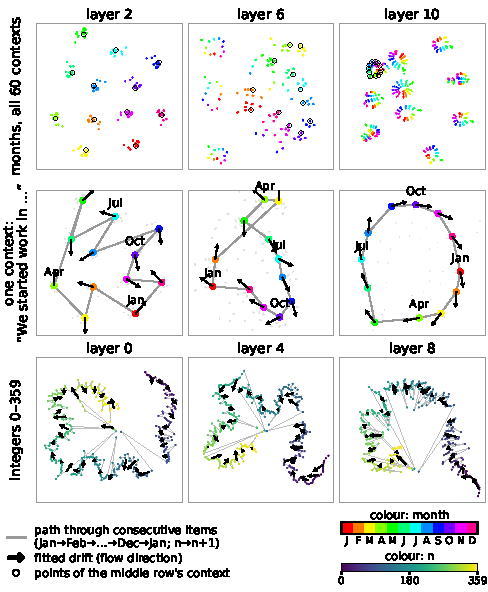
\includegraphics[width=\columnwidth]{figures/transformer_concepts.pdf}
  \caption{GPT-2 small, FlowSNE with a row-stochastic input; the input drift
  of each point is its successor in the same context. Arrows: fitted drift
  in flow direction. Grey line: the path through consecutive items
  (January$\to\dots\to$December$\to$January, $n\to n+1$).
  \emph{Top:} the 12 months at the end of 60 sentence contexts, at layers 2,
  6 and 10; the context of the middle row is circled. \emph{Middle:} that
  context alone: its months are scattered over the month clusters at layer
  2 and form a ring in calendar order by layer 10, which the drift turns
  around. \emph{Bottom:} integers 0--359 (mean over 10 contexts): one line
  with a wiggle per decade, the drift running along it; the straight grey
  segments are the jumps $10k{-}1\to 10k$ into the cluster of multiples of
  10 at the centre.}
  \label{fig:transformer}
\end{figure}

\todo[inline]{Section 6.3 text: setting (GPT-2 small, concept token,
successor drift), probe: last digit decodable but categorical, no helix in GPT-2 small (last-digit centroids equidistant); 3-D maps form no coil, rings already in
symmetric t-SNE (winding 0.88--1.00 vs 0.25--0.55 shuffled), FlowSNE
orients them (succ.\ cos 0.61--0.84, turning agrees 83--100\%), Finsler
t-SNE picks $\alpha=0$; numbers = gradient regime; residual-update drift is
${\sim}90\%$ constant (gauge). One seed so far.}
